\documentclass[hidelinks,a4paper,12pt]{article}
\addtolength{\oddsidemargin}{-1.cm}
\addtolength{\textwidth}{2cm}
\addtolength{\topmargin}{-2cm}
\addtolength{\textheight}{3.5cm}
\newcommand{\HRule}{\rule{\linewidth}{0.5mm}}
\makeindex

\usepackage{longtable}
\usepackage[pdftex]{graphicx}
\usepackage{makeidx}
\usepackage{hyperref}
\hypersetup{
    colorlinks=true,
    linkcolor=black,
    filecolor=blue,      
    urlcolor=blue,
}


% define the title
\author{Men-at-Work}
\title{ OnlyRugby Mobile Application User Manual}
\begin{document}
\setlength{\parskip}{6pt}

% generates the title
\begin{titlepage}

\begin{center}
% Upper part of the page       

\includegraphics[width=1\textwidth]{./images/up-logo.jpg}\\[0.4cm]    
\textsc{\LARGE Department of Computer Science}\\[1.5cm]
\textsc{\Large COS 301 - Software Engineering}\\[0.5cm]
% Title
\HRule \\[0.4cm]

\includegraphics[width=0.05\textwidth]{./images/logo.jpg} 
{ \huge \bfseries Amazon}

\includegraphics[width=0.05\textwidth]{./images/logo.jpg}\\[0.4cm] 
{ \huge \bfseries Network Visualizer}\\[0.4cm]
{ \huge \bfseries Demo 3}\\[0.4cm]
\HRule \\[0.4cm]
% Author and supervisor
\textsc{\Large Not-Like-This}\\[0.5cm]
\begin{minipage}{0.4\textwidth}
\begin{flushleft} \large
\emph{Authors:}
\end{flushleft}
\end{minipage}
\begin{minipage}{0.4\textwidth}
\begin{flushright} \large
\emph{Student number:}
\end{flushright}
\end{minipage}

\begin{minipage}{0.4\textwidth}
\begin{flushleft} \large
Jedd {Schneier}
\end{flushleft}
\end{minipage}
\begin{minipage}{0.4\textwidth}
\begin{flushright} \large
\emph{}
u13133064
\end{flushright}
\end{minipage}

\begin{minipage}{0.4\textwidth}
\begin{flushleft} \large
Daniel {King}
\end{flushleft}
\end{minipage}
\begin{minipage}{0.4\textwidth}
\begin{flushright} \large
\emph{}
u13307607
\end{flushright}
\end{minipage}

\begin{minipage}{0.4\textwidth}
\begin{flushleft} \large
Muller {Potgieter}
\end{flushleft}
\end{minipage}
\begin{minipage}{0.4\textwidth}
\begin{flushright} \large
\emph{}
u12003672
\end{flushright}
\end{minipage}

\vfill
% Bottom of the page
{\large \today}
\end{center}
\end{titlepage}
\footnotesize
%\input{declaration_of_originality.tex}
\normalsize


\pagenumbering{roman}
\tableofcontents
\newpage
\pagenumbering{arabic}

\newpage
\section{Vision} 
The Network Visualizer is intended to be used by registered Amazon Web Services (AWS) users. The visualizer is primarily aimed at consumers of AWS, in order to provide a simple and clear representation of the various networks' structures.

In order to access the visualizer, the user must first submit their AWS password and secret password. The visualizer then attempts to access the server, using the provided passwords. If this is successful, the visualizer will scan the specified network and log the nodes (such as instances and VPC's) and their relationships. It uses this information to construct a tree-esque representation of the network.

Using this representation, it is then translated into HTML. Making use of the vis.js library, the structure of the network is presented in a clear, visual hierarchial structure. The page also allows the user to specify which region they wish to be scanned and represented.

\section{Scope}
\begin {itemize}
	\item The user requires a valid Amazon Web Services account (or access to one), in order to make use of the visualizer.
	\item The user requires an internet capable device and a modern browser to access the visualizer's page.
\end{itemize}
\newpage

\section{Architectural Requirements}

\subsection{Architecture Scope}
Layered Architecture: 
RESTFUl Architecture
Threading Pool tactic:

\includegraphics[width=1.00\textwidth]{./images/layered.png}\\[0.4cm] 

\subsection{Quality Requirements}
\subsubsection {Critical}
\begin{enumerate}  
	\item Performance: The first and perhaps most important requirement. The system is working with massive amounts of data. The system is redundant if it can not process and show the data quickly. The majority of our architectual design has been done to improve performance. To keep it within its 3 second output requirement. 
	\item Scalability: This is one of the major quality requirements for the service, as stated before. The system will have to work with very large networks in future and thus, the algorithms within will need to scale well, such that they can work with these large networks and so that performance costs are minimized. So far, our performance requirements matches our scale.
\end{enumerate}		
\subsubsection {Important}
\begin{enumerate}  
	\item Security: From our own experince, we know how important security is with this system. As we are working with sensitive client info (links to credit cards), it is imperative that we make sure the system is secure and does not allow for this information to fall in the hands of unwanted 3rd parties or be compromised in any way.
	
	\item Usability: Usability is very important, as ease of use is imperative to the client's experience. However, it is not as important as performance or scalabilty; as at higher levels, regardless of usability the system will be required to meet those requirements. The system is going to be used by the Amazon clients who will not necessarily have programming knowledge, thus the end product needs to cater to these users.
\end{enumerate}	

\subsubsection {Nice To Have}
Maintainability: The system is going to be used by the Amazon clients who will not necessarily have programming knowledge, thus the end product needs to be catered to these users such that they are able to use the program efficiently.
\subsection{Architectural Constraint}
The user must have an existing and valid account with the Amazon services.The user must use a virtual network. The must have a valid credit card to set up their account. The user must have a relatively stable, preferably uncapped, internet connection. The user must also set up an access key and secret key on their end.
\subsection{Access and integration channels}
The information regarding the networks is taken via the Amazon API services.
\begin{itemize}  
	\item The user should login via the existing Amazon site and the visualizer should integrate into the site itself.
	\item The Front end must integrate through the REST server with the backend.
	\item The scanner must integrate with the Shared Buffer.
	\item The Scanner mustt integrate with AWS.
	\item The interface must integrate on all browsers and with standard web technologies
\end{itemize}

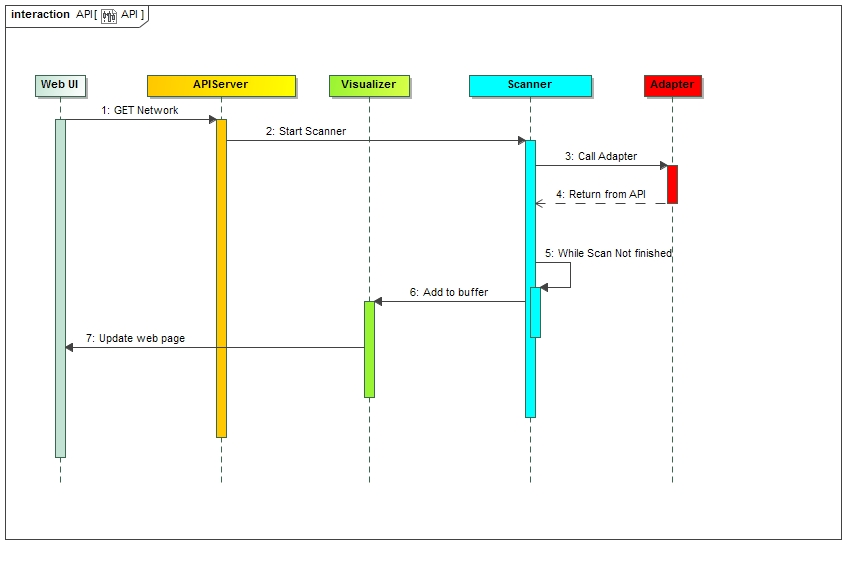
\includegraphics[width=1.00\textwidth]{./images/API.jpg}\\[0.4cm] 
\newpage
\section{Architectural Design}
\subsection{Layered Architecture} 

Our core architectural design follows a standard Client-Application-Server layered architecture. As seen below, the "Server" (not to be confused with the Application server) is the AWS server we connect to through their API. The product does not persist to only read from it and we have no control over its functionality. It will be left for an intergration requirement and will not be disccussed further in this section. Additional information on the AWS sytem and their API can be found here: \url{https://aws.amazon.com/documentation/}. Previously we used a  bridging layer, Adapter, to join the Application and Server layer, but  it has since been incorporated into the Scanner, to reduce communciation overhead and facilitate threading tactics.The primary backend of the system lies on the Application layer, which is broken down into the follwoing components:
\begin{enumerate}  
	\item Scanner: The most important component, constructs a scan based on different priorities. It forms a Producer-Consumer relationship with the Visualizer. Once launched, it will continue to produce network trees (see below) for the buffer until it receives a pause/stop command, or completes a scan of the network. 
	\item Composite:  Following the composite design pattern, this object represents the hierarchial Network tree, either in part or in whole.  
	\item Threaded Sub-Scanners: Each logical part of an AWS network has an assigned threaded scanner to it. Depending on what is a priority to scan first, the scanner will launch a number of threads for each part, which will in turn launch its sub-scan threads; based on performance requirements. Each threaded Sub-Scanner will scan 100 of it's children, place them in a buffer and then continue to scan another 100. 
	\item Smart buffer: The link between the Visualizer and the Scanner as well as the "brain" of the system. The individual scanner threads will add to the buffer as soon as they have finished constructing a tree, then go back to scanning. The trees arrive disjointed and possisbly overlap. The smart buffer constructs the entire network tree from the disjointed trees it receives accurately. It stores the most up to date construct for the Visualizer.
	\item REST API and Server: The REST server joins the back-end to the front-end. See architecture below.
\end{enumerate}

The client layer consists of a single page Application and the Visualizer. The SPA is the user interface with all the scanning options and control and the visualized graph and scanned information. The Visualizer polls on the REST server requesting the latest tree from the smart buffer, rendering it and presenting it to the user.

\subsection{RESTFUL Design}

User interaction is mapped from the user interface onto diffennt API calls, on the server. Each call launches a back-end method to fullfill the request. The API calls are:
\begin{enumerate}  
	\item POST, ConnectToAccount: Takes the users' access and private key and creates a connection to AWS for the remainder of the session.
	\item GET, ScanNetwork: Launches a scan of the entire network, Visualizer polls on results as they stream in. 
	\item GET, StopScan: Cancels the current scan.
	\item GET, PauseScan: Pauses the current scan.
	\item GET, ResumeScan:Resumes the current scan. Visualiser polls on buffer.
	\item GET, ScanFrom: Performs a subscan starting from the given point and scanning around its general vicinity.
	\item GET, ScanUP: Scans the next logical area above what the ScanFrom scanned.
	\item GET, ScanDown: Scans the next logical area below what the ScanFrom scanned.
\end{enumerate}

\subsection{Threading Tactic}
Each network component (Region,VPC,Sub-network,Instance) has a threaded scanner associated with it. It is up to the Scanner, depending on what the user is searching for, to construct the scan from the subscanners.
By defualt, the scanner will thread a RegionScanner for each region and each one will have one scanner for the other parts. However, if the scan is narrowed, then scanner will thread on the most cost and performance effective way to complete the scan . For example, if the scan was to only scan a single VPC then other Regions would not need to be scanned and thus only one RegionalScanner will be launched, one VPCScanner will be launched with a thread on collections of its subnetworks. We are trying to keep number of threads needed to a mninimum, but they are invaluable to speeding up the scanning.  



\newpage
\section{Functional Requirements}
	This section specifies the functional specifications for the AWS Network Visualizer system. It defines the user-system interaction and relationship between users and the product. It will provide the expected functionality for all user cases as well as the activity processes for the system.
	
		\subsection{Description of AWS}
			Amazon web services provide a cloud based service for hosting a clients network. There is a lack of information regarding one's network, specifically the logical representation on the system for the client to make sense of their network. The network visualizer aims to improve clients' understanding of their own network, how AWS works and possible insights in the managing of their network.
		\subsection{Required Functionality}
			The system must be able to:
				\begin{enumerate}  
					\item Be accessible to registered, valid AWS customers.
					\item Scan the networks located in different regions. 
					\item Provide an interactive hierarchical and visual representation of the networks.
					\item Give additional information on the network statistics, construction, etc.
					\item Provide a clear image of the clients' virtual networks.
					\item Improve the AWS clients' experience.
				\end{enumerate}
				
		\subsection{Use case}
		The usage of the system will typically consist of passing credentials to the system in the form of users' access and private key for their AWS account. If valid the system will ask the user to choose a region to be scanned. All artefacts in that region will be scanned and a network representation will
		be constructed that will be displayed to the user. The representation can also be interacted with to expand nodes and request further information.
		
		\subsection{Use case/Service contracts}
		\begin{tabular}{ | p{3cm} | p{4cm} | p{4cm} | p{4cm} |}
			\hline
			Use Case & Pre Condition & Post Condition & Description \\ \hline
			
			Viewing the Hierarchy & The application must be connected to the server and able to read in network data. The server must be active and have access to AWS.& The web page continuously updates with the new data being loaded. & This use case forms the core of the project, as the primary purpose of the application is to visualise the structure of the virtual network.\\ \hline
			
			Select a region 	& The application must be connected to the server and able to read in network data. The server must be active and have access to AWS.& The previous region's visualisation is replaced by the selected region. & There are a number of AWS regions. For simplicity's sake, the visualiser only visualises one at a time, but allows for switching between them.\\ \hline
			
			Zooming in/out. Moving the hierarchy	& The application must be connected to the server and able to read in network data. The server must be active and have access to AWS.& The hierarchy's position or level of zoom is altered. & Since the visualised network may be large, the user can move it about and zoom in, for a better view.\\ \hline
			
			Clicking a node.& The application must be connected to the server and able to read in network data. The server must be active and have access to AWS.& The selected node is highlighted. Node related information is displayed below the hierarchy. & Each node in the network has a number of attributes that can provide valuable information. This way, the information can be displayed in a neat manner.\\ \hline
			
			Hovering over a node.& The application must be connected to the server and able to read in network data. The server must be active and have access to AWS.& Edges connecting nodes of different levels are rendered invisible. Edges connecting nodes on the same level are made visible. & It is possible for nodes on the same level of the network to have relationships. They are normally hidden, in order to present a cleaner hierarchy. \\ \hline
		\end{tabular}
\newpage		
\subsection{Using the System}		
	\subsubsection{Login}
	\textbf{Description}
	\newline
	This function validates clients' credentials to allow them to scan an accounts network.
	\textbf{Inputs}
	\newline
	Client’s access key and client’s private key.
	\newline
	\textbf{Processing}
	\newline
	The access key and private key is passed to a Credentials object. The credentials are validated by
	trying to connect to an account with those keys.
	\newline
	\textbf{Outputs}
	\newline
	If validation successful:
	\newline
	Access to the visualization interface.
	\newline
	If invalid:
	\newline
	Error message and retry prompt.
	\newline
	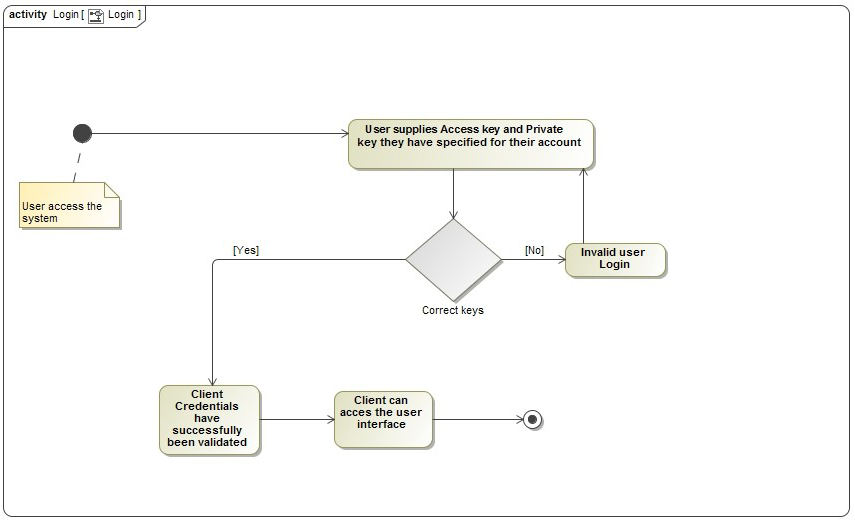
\includegraphics[width=1.00\textwidth]{./images/Login.png}\\[0.4cm] 
	\newpage	
	\subsubsection{Scan Network}
	\textbf{Description}
	\newline
	This function scans the user’s networks in a specified region.
	\textbf{Inputs}
	\newline
	Specified region and filtering options to limit the data desired.
	\newline
	\textbf{Processing}
	\newline
	The scanner connects through the adapter interface, makes the desired API calls and constructs a
	representation object of the network
	\newline
	\textbf{Outputs}
	\newline
	If no exceptions:
	\newline
	The visualization application will be passed a Network object to render.
	\newline
	If exception thrown:
	\newline
	Error message, log the problem take user back to interface.
	\newline
	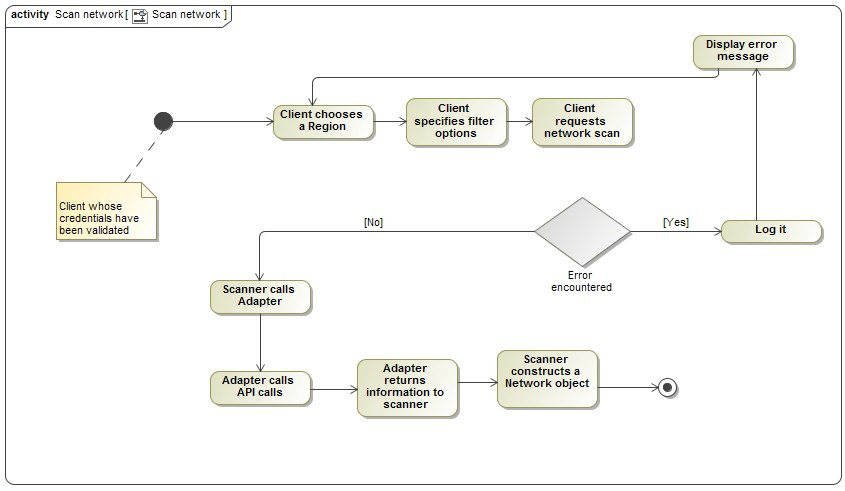
\includegraphics[width=1.00\textwidth]{./images/Scan.png}\\[0.4cm] 
	\newpage	
	\subsubsection{Visualise Network}
	\textbf{Description}
	\newline
	This function graphically renders the network.
	\textbf{Inputs}
	\newline
	Constructed Network object from scanner.
	\newline
	\textbf{Processing}
	\newline
The visualizer recursively traverses the Network object, creating a tree hierarchy and rendering it for the user.
	\newline
	\textbf{Outputs}
	\newline
	If no exceptions:
	\newline
	A fully rendered representation of the network.
	\newline
	If exception thrown:
	\newline
	Error message, log the problem take user back to interface.
	\newline
	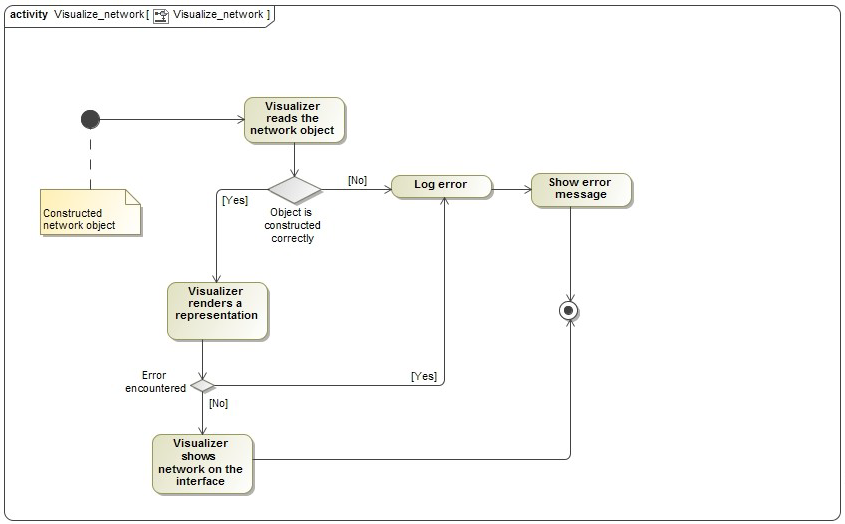
\includegraphics[width=1.00\textwidth]{./images/Visualise.png}\\[0.4cm] 
	\newpage	
		\subsubsection{Expand Information}
		\textbf{Description}
		\newline
		This function produces a dialogue of additional information for selected node.
		\textbf{Inputs}
		\newline
		User clicks desired node.
		\newline
		\textbf{Processing}
		\newline
		The system will retrieve additional information on the desired node and return it to the interface.
		\newline
		\textbf{Outputs}
		\newline
		If no exceptions:
		\newline
		Additional information will be shown
		\newline
		If exception thrown:
		\newline
		Dialogue shows no additional information, log the error, show an error message in dialogue.
		\newline
		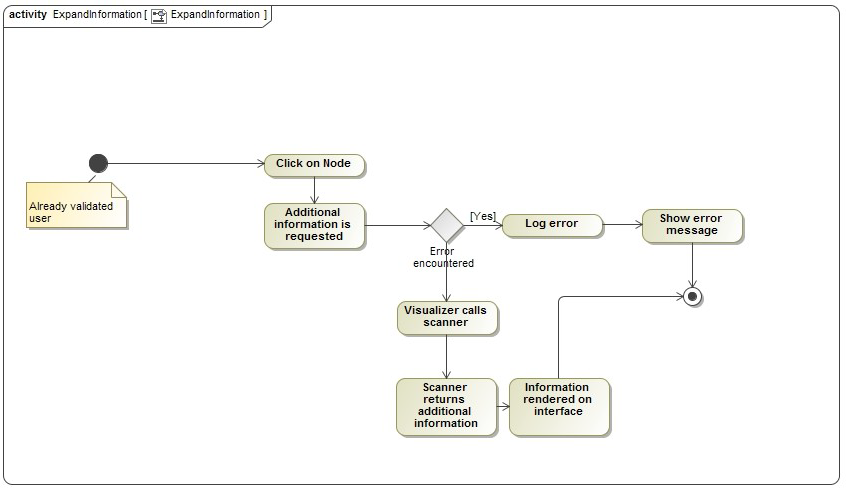
\includegraphics[width=1.00\textwidth]{./images/ExpandInformation.png}\\[0.4cm] 
	
	
	
\newpage
\section{Specification Update}
	The specification has remained largely unchanged. The initial task of creating a high speed network scanner has not changed, however it has been reworked as a plugin, which will allow for easier deployment.
\section{Testing}
	Sadly, our system is not yet at a point where it can be properly tested


















	

\end{document}
